%%%%%%%%%%%%%%%%%%%%%%%%%%%%%%%%%%%%%%%%%
% Template for Logical Writing Final Report 2022.
% Template Written by Heejun Lee
% Content provided by Prof. Seo Yun Jung
% Created: 2022/12/06
% Updated: 2022/12/06
% Tested on Overleaf with XeLaTex 2022
%%%%%%%%%%%%%%%%%%%%%%%%%%%%%%%%%%%%%%%%%
%       Beginner TODOs
% 1. Change Title / Author in main.tex
% 2. Write your abstract text in sections/abstract.tex
% 3. Write your body text in sections/body.tex. You are freely adding more sections and splitted files using \input command.
%%%%%%%%%%%%%%%%%%%%%%%%%%%%%%%%%%%%%%%%%
%       Beginners Guide for Figure
% For figure inside of body text, you can find example in /figures folder. Figure should be splitted into two file 'tex' and 'image' files. This is convenient way to manage your tex definition and actual image. I suggest you to add figure image in format 'pdf'.
%%%%%%%%%%%%%%%%%%%%%%%%%%%%%%%%%%%%%%%%%
%       Beginners Guide for Reference
% The auto-referencing is the main feature of latex. This is why I am creating this template... with my own efforts. You can reference any figures and tables by given label with `\ref{fig_name}`. You can give figure name with `\label{fig_name}`. You can find the example of this inside of body.tex.
% Not only auto reference figures and tables, you can cite automatically, without considering order of citation. Latex will automatically sort your citation and format in APA style. WOW! example is `\cite{google}`. You can find example in body.tex. And you should add reference information in BibTex form into `refs.bib`.
%%%%%%%%%%%%%%%%%%%%%%%%%%%%%%%%%%%%%%%%%

\documentclass[a4paper,10pt,twocolumn]{article}
\usepackage{indentfirst}
\usepackage[utf8]{inputenc}
\PassOptionsToPackage{no-math}{fontspec}
\usepackage{xltxtra}
\usepackage{xeCJK}
\xeCJKsetup{
    CJKspace=true,
    CJKecglue={}
}
\setmainfont{Noto Serif}
\setCJKmainfont{Noto Serif CJK KR}
\setCJKsansfont{Noto Sans CJK KR}
\setCJKmonofont{Noto Sans Mono CJK KR}
\usepackage{setspace}
\usepackage{cuted}

\usepackage[bitstream-charter]{mathdesign}
\usepackage{ragged2e}
\usepackage[%
    backend=bibtex      % biber or bibtex
    %,style=authoryear    % Alphabeticalsch
    ,style=numeric-comp  % numerical-compressed
    ,sorting=none        % no sorting
    ,sortcites=true      % some other example options ...
    ,block=none
    ,indexing=false
    ,citereset=none
    ,isbn=true
    ,url=true
    ,doi=true            % prints doi
    ,natbib=true         % if you need natbib functions
    ,backref=true
]{biblatex}
\DefineBibliographyStrings{english}{%
  backrefpage = {page},% originally "cited on page"
  backrefpages = {pages},% originally "cited on pages"
}
\addbibresource{refs}  % better than \bibliography
\usepackage{authoraftertitle}
\usepackage[
    colorlinks=true,
    allcolors = black,
    citecolor=blue, 
]{hyperref} 

\usepackage{anyfontsize}
\usepackage{anysize}
\usepackage{amsmath}
\usepackage{textcomp,gensymb}
% \usepackage{float}
\usepackage{lipsum}
\usepackage{graphicx}
\usepackage{graphics}
\usepackage[font=small,labelfont=bf]{caption}
\usepackage{subcaption}
\usepackage{url}
\usepackage{multicol}
\usepackage{float}
\usepackage{titlesec}
\usepackage{adjustbox}
% \usepackage{dblfloatfix}
% \usepackage{stfloats}

%%%%%%%%%%%%%%%%%%%%%%%%%%%%%%%%%%%%%%%%%%%%%%%%%%%%
%   For change page format
%%%%%%%%%%%%%%%%%%%%%%%%%%%%%%%%%%%%%%%%%%%%%%%%%%%%
%Page margin
\marginsize{0.6in}{0.6in}{0.6in}{0.6in}
%Two column margin
\setlength\columnsep{0.33in}
%Abstract format
\renewenvironment{abstract}
 {\par\noindent\textbf{Abstract}\ \ignorespaces \\}
 {\par\noindent\medskip}
%double line for abstract
\newcommand{\doublerule}[1][.4pt]{%
  \noindent
  \makebox[0pt][l]{\rule[.7ex]{\linewidth}{#1}}%
  \rule[.3ex]{\linewidth}{#1}}
%Font setting for section
\titleformat*{\section}
    {\fontsize{11pt}{11}\bfseries} 
%Font setting for subsection
\titleformat*{\subsection}
    {\fontsize{10pt}{10}\bfseries}
%Font setting for subsubsection
\titleformat*{\subsubsection}
    {\fontsize{10pt}{10}\bfseries}
%Korean for figure
\renewcommand{\figurename}{그림}
%Default line height
\setstretch{1.5}
\captionsetup[table]{font={stretch=1.3}}
\captionsetup[figure]{font={stretch=1.3}}

%%%%%%%%%%%%%%%%%%%%%%%%%%%%%%%%%%%%%%%%%%
% TODO: Change this metadata for change your title.
%%%%%%%%%%%%%%%%%%%%%%%%%%%%%%%%%%%%%%%%%%%
\title{논리적 글쓰기 \Large{\LaTeX}~템플릿}
\author{이희준\\Undergraduate School of Computing\\Korea Advanced Institute of Science and Technology (KAIST)}

\begin{document}
\begin{strip}
\vspace{-1in}
\begin{center}
\setstretch{1.15}{
\textbf{\fontsize{13pt}{13pt}{\MyTitle}} \\
\vspace{1em}
\textbf{\fontsize{11pt}{11pt}{\MyAuthor}}
}
\medskip

\normalsize

\end{center}
\doublerule
\vspace{0.2cm}
\begin{abstract}
\fontsize{9pt}{9pt}
국문 혹은 영문 초록을 쓰는 부분이다. 연구 목적, 연구 결과, 연구의 의의 및 활용 방안을 간결하게 작성한다. 이 과제에서는 국문 초록을 작성하면 된다(공백 포함 300자 이내).

\medskip
\noindent
핵심어: 스트레스, 식비, 선형 회귀, PCA
\end{abstract}
\doublerule
\end{strip}
\section{서론}
\begin{figure}[H]

\includegraphics[width=\linewidth]{images/cats.jpg}
\caption{이건 작은 피겨이다. 구글에서 아무 이미지나 가져왔다. 이렇게 설명문 안에서도 참조 할 수 있다~\cite{texbook}.}
\label{fig:small}
\centering
\end{figure}

서론은 주요 연구 대상과 관련된 개념, 연구 주제와 관련된 배경 정보, 관련 연구(선행 연구)를 기술한 후, 연구 목적을 제시하는 것이 일반적이다. 이때 연구 목적에 대한 당위성을 설정하는 것이 중요하다. 제안서에 작성하면서 연구 가설을 세웠기 때문에 이를 서론에서 적절히 언급해 주고, 이 가설을 검증하기 위한 연구 방법을 소개하는 것으로 자연스럽게 2장을 전개하는 것이 좋다.

선행 연구에 대한 인용 표기의 첫 번째 방식은 이와 같다~\cite{google}. 선행 연구의 인용 표기의 두 번째 방식은 다음과 같다~\citep{texbook}. 두 유형의 인용 방식 중 하나를 선택하여 사용한다. 각주는 다음과 같은 방식으로 사용한다. 각주의 기능은 각주 1을 참고하면 된다.

(폰트는 바탕을 권장. 줄 간격 1.15. 장 제목 11pt, 절 제목 10pt, 본문 10pt로 작성. 장과 장/절 사이에는 엔터를 넣어 구분.)

\section{연구 방법}
연구 자료는 연구 목적을 달성하기 위해 사용한 자료를 소개하는 장이다. 일반적으로 자료 제반에 대한 설명(구성 방식, 규모, 구축 기간, 참가자 정보 등)을 하되 샘플을 중심으로 기술하는 것이 좋다.

분석 방법론이 특별할 경우 장을 따로 설정하여 기술한다. 2장의 하위 절은 연구 목적과 연구자의 스타일에 따라서 다양하게 구성할 수 있다. 

\subsection{연구 자료}
식사 DB의 전반적 구성을 설명하는 절이다. DB의 대상, 규모, 수집 정보의 하위 분류 등을 상세히 설명해야 한다. 연구자가 직접 수집한 자료가 아니기 때문에 수집 방법을 설명할 필요는 없으며, 기구축된 자료를 사용하여 분석을 진행하였음을 기술해 주면 된다. 

아래의 <그림 \ref{fig:small}>은 원래 식사 DB의 예시었던 고양이들이며, 이렇게 데이터의 구성을 독자들에게 보여주는 것이 가능하다. 그러나 지면의 제약이 크기 때문에 반드시 DB를 이미지로 소개할 필요는 없다.

\subsection{분석 방법}
분석 방법은 자료를 처리한 과정(자료 재처리, 프로그램 등)을 기술하는 절이다. 만약 DB를 가공하여 연구를 진행한 경우에는 어떠한 기준으로 데이터 토큰을 제외하였는지 명확히 제시해야 하며, 그 결과 몇 개의 토큰이 제외되었으며, 분석 대상으로 삼은 최종 데이터 수를 기술해야 한다. 

특별한 방법론을 사용했거나 특정 프로그램을 사용했다면 반드시 기술해야 한다. 이 과제를 수행하는 데 사용한 특별한 방법론이 없다면 기술하지 않아도 되지만 간단하게라도 써 보도록 하자.

\section{연구 주제를 기반으로 장 제목 제시}

\subsection{절 제목 = 연구의 핵심}

\subsection{필요하다면 장과 절을 더 세분하여 기술해도 됨}

3장부터는 분석 결과를 제시하고 그에 대한 논의를 진행한다. 데이터를 일목요연하게 보여줄 수 있는 표와 그래프를 제시하는 것을 권장하나, 이러한 표와 그래프만으로 보고서를 채우는 것은 지양해야 한다. 표의 크기가 큰 경우에는 2단에 걸쳐 제시하는 것이 가능하다. 

표와 그래프 아래에는 반드시 그 차트를 설명하는 단락이 있어야 한다. 차트를 읽는 방법을 설명하고, 주목해야 할 만한 부분을 설명해 주어야 한다. 강조하고 싶은 부분에 음영이나 강조색을 넣는 것도 좋은 방법이다.

단순히 분석 결과만 제시해서는 안 되며, 그 결과에 대한 연구자의 해석을 제시해야 한다. 가능한 한 범위에서 논의를 진행해야 하며, 성급한 일반화의 오류를 범하지 않도록 주의를 해야 한다. 우리가 연구 대상으로 삼은 DB는 여러 가지 한계를 품고 있음을 언제나 명심해야 한다.

논의는 연구 결과와 같은 장에서 기술하는 것이 가능하나, 결과와 논의가 혼재되지 않도록 분명히 구분하여 작성하여야 한다. 논의를 결론과 같은 장에서 기술하는 것도 가능하다. 그렇지만 이 과제에서는 논의를 풍부하게 기술하도록 권장하고 있으므로 논의를 먼저 제시하고 결론을 내리는 방식으로 구성하는 것이 좋다. 물론, 연구 결과와 논의, 결론을 모두 별개의 장으로 작성하는 것도 가능하다.

\section{결론}
% \begin{figure}[!t]
% \centering
% 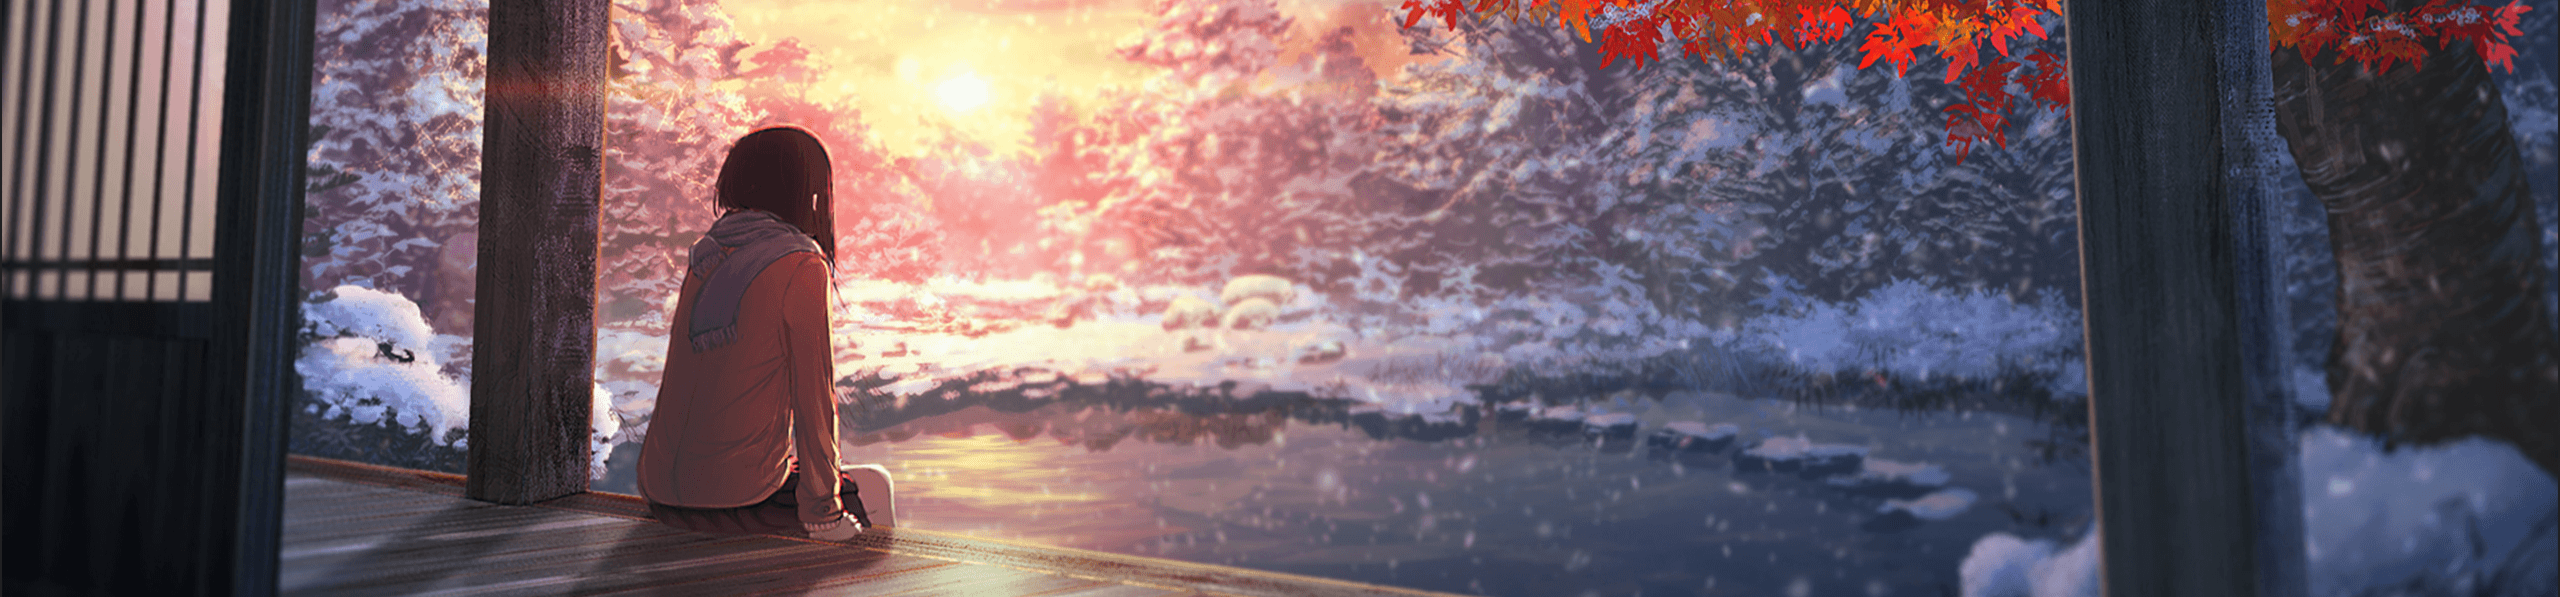
\includegraphics[width=\textwidth, height=5cm]{images/wide.png}
% \caption{이건 넓은 피겨이다. 구글에서 아무 이미지나 가져왔다. 이렇게 설명문 안에서도 참조 할 수 있다~\cite{wide_wallpaper}.}
% \label{fig:wide}
% \centering
% \end{figure}

% \noindent
% 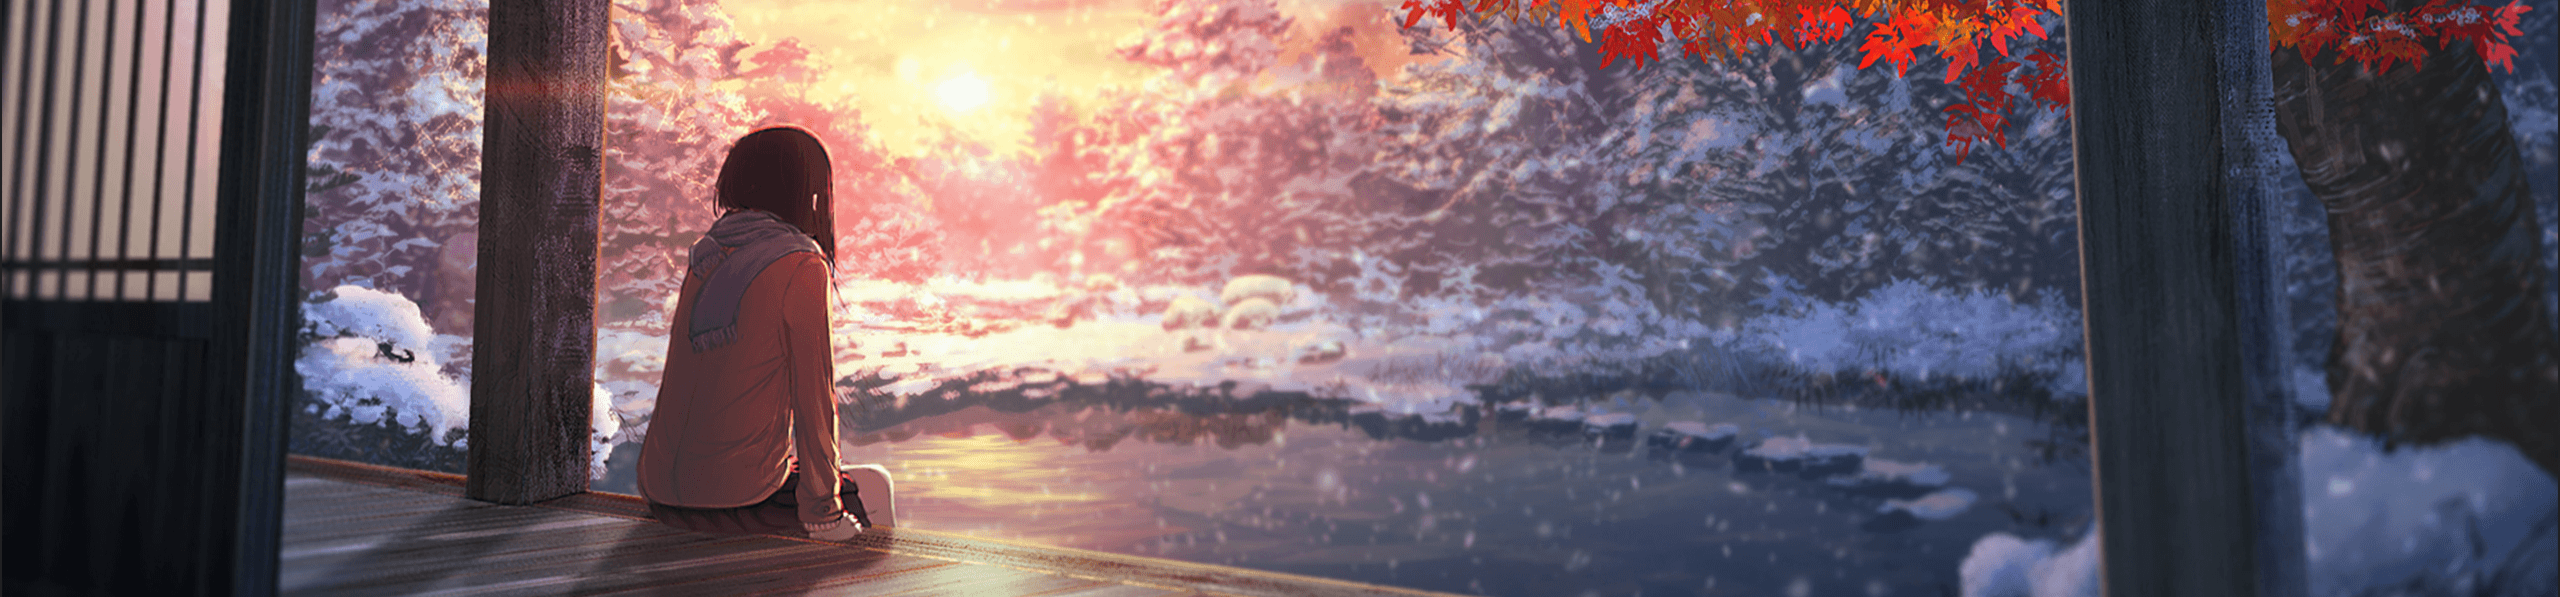
\includegraphics[width=\textwidth, height=5cm]{images/wide.png}

\vspace{1.0em}
\noindent
\begin{minipage}[!t]{\textwidth}%
\makebox[\linewidth]{%   For centring figures
    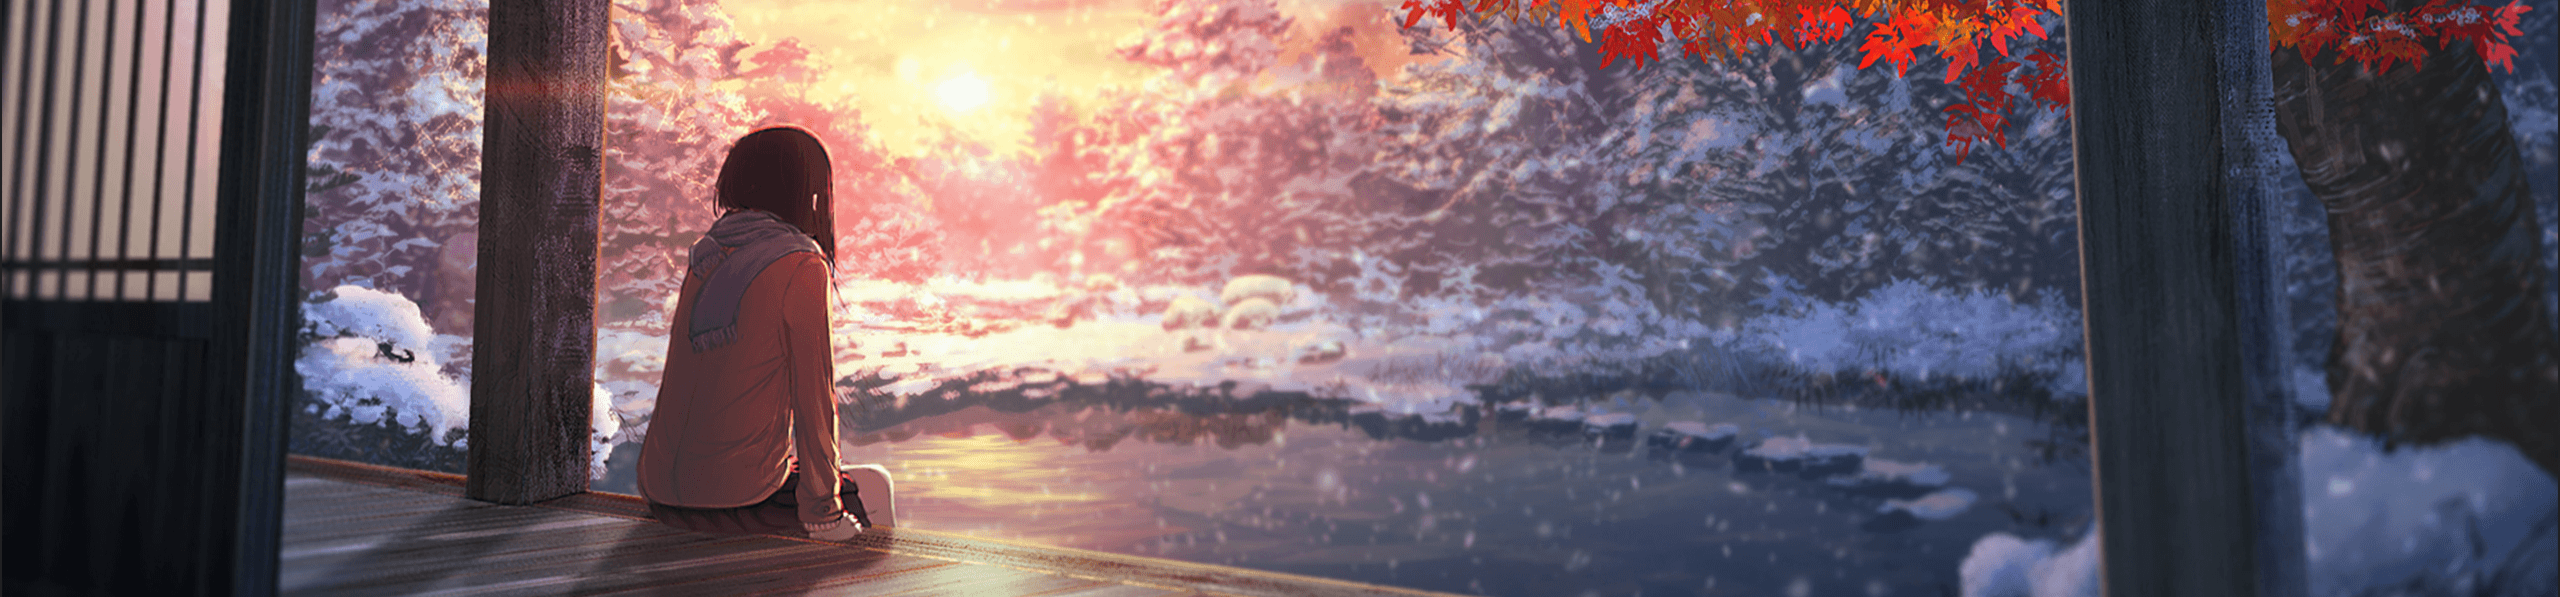
\includegraphics[width=\linewidth]{images/wide.png}
}
\captionof{figure}{
이건 넓은 피겨이다. 미니 페이지를 이용한 꼼수로 twocolumn에서도 페이지 단위의 피겨를 넣을 수 있다. 차후 개선이 필요하다. 구글에서 아무 이미지나 가져왔다. 이렇게 설명문 안에서도 참조 할 수 있다~\cite{wide_wallpaper}.
}
\vspace{1.0em}
\label{fig:wide}
\end{minipage}
결론은 연구 목적, 결과를 요약하고 연구의 의의를 제시하는 부분이다. 결론에는 전체 연구를 개괄하는 내용의 단락이 하나 존재해야 한다. 그리고 연구의 의의, 활용 방안은 결론의 꽃이다. 반드시 써야 한다. 의의와 활용 방안은 거시적 관점에서 기술하되 너무 추상적이지 않게 제시해야 한다. 그리고 이렇게 그림 \ref{fig:wide}를 참조 할 수 있다.

연구의 한계를 지적하면서 결론이 마무리되면 독자에게는 실패한 연구라는 인상이 강하게 남을 수 있다. 따라서 분명한 한계가 있었음에도 해 볼 만한 가치가 있는 연구였다는 식으로 독자를 설득하는 것이 좋다. 또한, 부족한 부분을 보완할 수 있는 방법을 제안하며 후속 연구를 기약하는 것도 또 하나의 방법이다.

\printbibliography

%%%%%%%%%%%%%%%%%%%%%%%%%%%%%%%%%%%%%%%%%
% start of appendix
\appendix
\setcounter{table}{0}
\renewcommand{\thetable}{\thesection.\arabic{table}}
\setcounter{figure}{0}
\renewcommand{\thefigure}{\thesection.\arabic{figure}}
\section{부록}

부록 테스트 텍스트. 부록이 필요없다면 \texttt{main.tex} 에서 부록 부분을 코멘트 처리하도록 하자.

\subsection{부록의 임시 챕터}

부록은 분량에 포함이 되지 않는다 한다.
% end of appendix
%%%%%%%%%%%%%%%%%%%%%%%%%%%%%%%%%%%%%%%%%
\end{document}